\documentclass{article}

% if you need to pass options to natbib, use, e.g.:
%     \PassOptionsToPackage{numbers, compress}{natbib}
% before loading neurips_2021

% ready for submission
\usepackage[preprint]{neurips_2021}
\bibliographystyle{plain}
% to compile a preprint version, e.g., for submission to arXiv, add add the
% [preprint] option:
%     \usepackage[preprint]{neurips_2021}

% to compile a camera-ready version, add the [final] option, e.g.:
%     \usepackage[final]{neurips_2021}

% to avoid loading the natbib package, add option nonatbib:
%    \usepackage[nonatbib]{neurips_2021}
\usepackage[pdftex]{graphicx}
\usepackage[utf8]{inputenc} % allow utf-8 input
\usepackage[T1]{fontenc}    % use 8-bit T1 fonts
\usepackage[hidelinks]{hyperref}       % hyperlinks
\usepackage{url}            % simple URL typesetting
\usepackage{booktabs}       % professional-quality tables
\usepackage{amsfonts}       % blackboard math symbols
\usepackage{nicefrac}       % compact symbols for 1/2, etc.
\usepackage{microtype}      % microtypography
\usepackage{xcolor}         % colors
\usepackage{cleveref}
\usepackage{float}
\usepackage{hyperref}
\usepackage[list=true, font=small, labelfont=bf, 
labelformat=brace, position=top]{subcaption}

\title{Analysis of german rental prices}

% The \author macro works with any number of authors. There are two commands
% used to separate the names and addresses of multiple authors: \And and \AND.
%
% Using \And between authors leaves it to LaTeX to determine where to break the
% lines. Using \AND forces a line break at that point. So, if LaTeX puts 3 of 4
% authors names on the first line, and the last on the second line, try using
% \AND instead of \And before the third author name.

\author{%
  Maximilian Hilbert, 4238218\\
  B. Sc. Physics\\
  University of Tübingen\\
  \texttt{\href{https://github.com/MaximilianHilbert/Data\_Literacy\_Project.git}{Github}}\\
  \texttt{maximilian.hilbert@student.uni-tuebingen.de}
}

\begin{document}
	\maketitle
\begin{abstract}
		An indication of an increasing spread between german rental prices is given by the analysis of 2 472 German districts (cities) that contain several years of historical data which depict a rise in inflation adjusted standard deviation between 2010 and 2017 of 19.5\% and an average increase of 13.5\%. In addition to that, there is a trend that lower priced housing vanishes and the distribution of rental prices develops a right handed heavy tail.
\end{abstract}

\section{Introduction}
	In past years, german rental prices soared. Frequently, it is argued that affordable rental homes vanish because modern and therefore higher priced flats are being built instead. To quantify this argument, a statistical approach is being done in the following. In order to answer the given question, data containing rental prices of 2 400+ german cities are provided by 1337 UGC GmbH on their website, as well as their mapping to the state where they are located in. \cite{rental_prices_city,rental_prices_states}
	
\section{Data aquisition using Regular Expressions (RegEx) and pandas}
\subsection{Gathering data: Rental prices of german cities}

	In the beginning, an examination on the overview of german cities \cite{rental_prices_city} is done to find out about the underlying problem of garnering data from the website. It turns out that a table of about 5 000 german districts is given. Each district is linked to a separate .html-file, containing more detailed information about historical rental prices in a java script line-graph. \\
	\\Unfortunately, only about 2 400 of these links are operational at the time of downloading, the remaining portion is either leading to a 404-error or other internal server errors. As a first step of the data acquisition process, a link search in the .html-file of the "main" page is being performed. This is followed by an automated download to get the required raw data files of each city mentioned on the website.
    
	Due to the fact that every district has a different amount of historical data, the widest interval of data provided had to be found. After inspecting the raw datafiles, it appears that the line-graph which shows the historical data always has the same css-id. \\\\
	Hence, a usage of RegEx was possible to find data provided directly succeeding this special css-id. The pattern search lead to the data, which is the rental price in EUR per $\mathrm{m^2}$. Of course these values are rental prices not containing any additional costs.\\\\
	The longest interval in the dataset is carried by Hannover and 6 other districts with data for years reaching from 2002 to 2017. The smallest interval is given by Lemberg and 16 other districts reaching only from 2009 to 2017.

\subsection{Gathering data: Matching cities to corresponding states}
	After the aquisition process of raw city data, a mapping dictionary between cities and states is being generated through a manual download of website content as .txt-files. \cite{rental_prices_states}\\\\
	Saving these files separately for each state and scanning with a specialized RegEx leads to a dictionary which maps all 16 german states to their corresponding city list. Finding a correct RegEx has been a serious challenge throughout the process, because there are several contradicting writing styles existing for german cities. \\\\
	Furthermore, common german special characters, like umlauts or the Eszett (ß), as well as citynames that are composed of up to three single words with whitespaces or even brackets in between, were challenges occuring in the process. Examples for such an edge case is "Bad Waldsee" or "Ellwangen (Jagst)".

\subsection{Data cleaning and processing}
	Having raw data aquired, it is now possible to generate dataframes, each different regarding its purpose of use. To get a general idea about the amount of data points garnered, the first operation is to sum up all data points unequal NaN that are contained in our dataset for every year. As mentioned before, the originally amount of about 5 000 cities has decreased to about 2 400. Furthermore, the timespan  from 2010 to 2017 is the only one being able to provide a sufficient amount of data points to perform a further statistical analysis. For detailed information see Table \ref{Table_raw}.

\renewcommand{\arraystretch}{1.3}
		\begin{table}[h!]
			\caption{Raw data containing a total of 22 000 data points from 2 400 german districts acquired from .html files. Note that the values are inflation adjusted. The provided data show, that there has been an increase in average rental prices in the timeframe from 2010 to 2017 of 13.5\% and 19.5\% in standard deviation, respectively.}
			\label{Table_raw}
			\centering
			\begin{tabular}{lrrlrrr}
\toprule
{} &  aach &  aachen &  ... &  Mean in $\mathrm{\frac{EUR}{m^2}}$ &  SD in $\mathrm{\frac{EUR}{m^2}}$ &  Historical data points \\
\midrule
2002 &   NaN &     NaN &  ... &                                5.48 &                              0.74 &                       8 \\
2003 &   NaN &     NaN &  ... &                                5.27 &                              0.77 &                      11 \\
2004 &   NaN &     NaN &  ... &                                5.66 &                              0.95 &                      15 \\
2005 &   NaN &     NaN &  ... &                                5.27 &                              0.74 &                      15 \\
2006 &   NaN &     NaN &  ... &                                5.22 &                              0.67 &                      17 \\
2007 &   NaN &     NaN &  ... &                                4.93 &                              0.79 &                      18 \\
2008 &   NaN &     NaN &  ... &                                4.91 &                              1.00 &                     135 \\
\vspace{0.3cm}
2009 &  6.68 &     NaN &  ... &                                5.55 &                              1.29 &                     410 \\
2010 &  5.14 &    6.95 &  ... &                                5.27 &                              1.28 &                    2254 \\
2011 &  5.68 &    7.19 &  ... &                                5.30 &                              1.25 &                    2382 \\
2012 &  5.97 &    7.63 &  ... &                                5.29 &                              1.29 &                    2392 \\
2013 &  5.09 &    7.92 &  ... &                                5.31 &                              1.34 &                    2406 \\
2014 &  6.53 &    8.16 &  ... &                                5.36 &                              1.33 &                    2399 \\
2015 &  6.37 &    8.30 &  ... &                                5.47 &                              1.31 &                    2458 \\
2016 &  6.69 &    8.64 &  ... &                                5.73 &                              1.38 &                    2449 \\
2017 &  7.04 &    8.87 &  ... &                                5.98 &                              1.53 &                    2471 \\
\bottomrule
\end{tabular}

		\end{table}
	\newpage
\section{Results and Visualisation}
\subsection{Visualisations of the entire dataset}
	\label{results}
	First of all, it can be said that the average increase in rental prices across germany seems not to be as servere as it typically gets displayed in the media. This conclusion can be made if one takes the inflation into account that has led to increasing prices in the last years. \cite{inflation}
	\\\\As this analysis is trying to find out about rising prices of rental housing, it is neccessary to adress the issue, that approx. 20\% of the official inflation rate consists of rental housing without additional expenses (ger.: Nettokaltmiete). \cite{inflation_ratio} 
	\\\\Therefore, a correction factor of 0.8 has been taken into account in order to achieve \cref{barchart_rental_prices}. Because the difference is smaller than thought in the first place, in further inflation adjustments the full adjustment (incl. rental housing) is being done.
	In order to be able to answer the thesis question whether lower priced rental housing vanishes in favor of higher priced ones, an analysis as shown in \cref{histogram_rental_prices} is neccessary.
	\\\\
	Here it comes obvious, that although the values have been fully inflation adjusted, a rise in average housing prices is not the issue, but the shift towards higher prices, whereas the supply of cheap housing starts to vanish. Overall the data shows, that lower rentals are vanishing in favor of higher priced ones. In addition to that, the differences between those categories also increase (higher standard deviation). This can be seen by the fact, that the whole distribution is moving to higher values and builds up a heavy tail towards higher priced rentals, while the tail on the lower cost side vanishes almost completely. In general it can be said, that the distribution seems to flatten out but more on the right hand side, than on the other.
	\\\\
	Diving deeper into the dataset, there are additional interesting insights that can be found. For instance, the data show that there is an indication of expensive cities being located most likely in Bavaria, especially in the Munich region. Furthermore, after grouping the dataset in favor of states the cities are located in, it can be seen that the eastern states (ger.: neue Bundesländer) tend to have lower priced rentals than western states (ger.: alte Bundesländer) do. This could be the case, because of several reasons, like differences in average income, borders to other countries, etc. These will not be discussed further in this paper.
		\begin{figure}[htp]
			\centering
			\includegraphics[width=0.7\linewidth]{../fig/figures/barchart_rental_prices.pdf}
			\caption{Inflation adjusted average prices and standard deviations across the dataset reaching from 2010 to 2017, containing a minimum of 2 200 data points in 2010 and a maximum of 2 400 in 2017.\\It can be seen that the dynamics of increasing rental prices start in 2015 and the trend is becoming interesting towards the end of the period supplied by the data. In favor of a clearer view onto the data, only errorbars for the partially adjusted means have been given.}
			\label{barchart_rental_prices}
		\end{figure}
	
		\begin{figure}[htp]
		\centering
		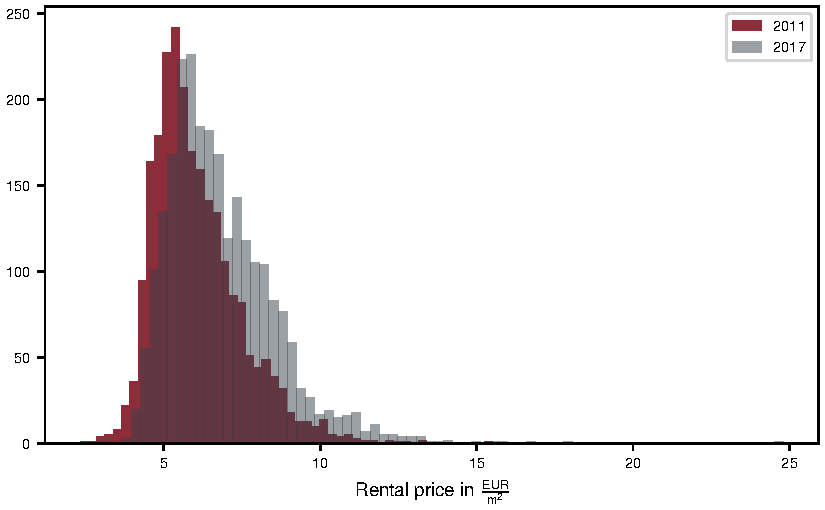
\includegraphics[width=0.7\linewidth]{../fig/figures/Histogram_rental_prices.pdf}
		\caption{Histogram on the frequency of appearance for rental prices in the dataset for 2011 and 2017. Values for 2017 have been fully inflation adjusted as mentioned in \cref{results}. It can be seen that the distribution for both years show a "heavy tail" for higher prices. Furthermore, a higher peak and a shifted mass towards higher prices can be seen for 2017. Note that the year 2011 has been chosen for comparison, because of the fact, that the number of data points is better comparable, see \cref{Table_raw}.}
		\label{histogram_rental_prices}
		\end{figure}


	\begin{figure}[htp]
	\centering
	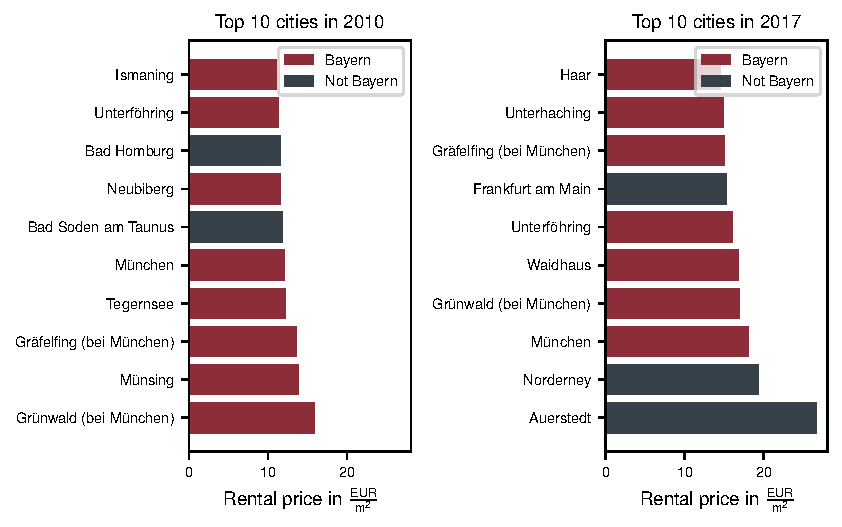
\includegraphics[width=0.9\linewidth]{../fig/figures/barchart_city_comparison.pdf}
	\caption{The dataset shows that almost all of the top 10 highest priced cities are located in Bavaria and three of them are in the region of Munich. Furthermore, the islands in northern Germany show a great rental price. This could be the case, because of a lack in the provided data.}
	\label{barchart_city_comparison}
	\end{figure}

	\begin{figure}[htp]
	\centering
	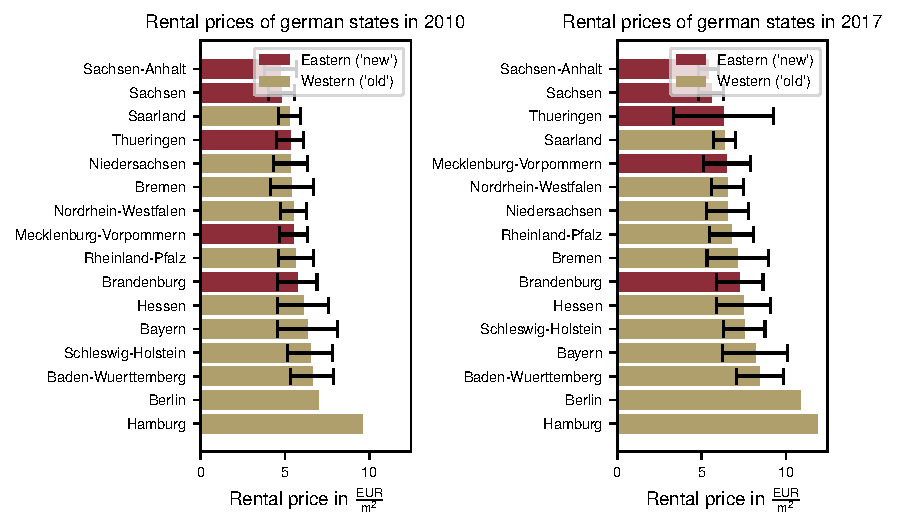
\includegraphics{../fig/figures/barchart_state_comparison.pdf}
	\caption{Averages and standard deviations for german states, achieved by grouping the raw dataset by states. Note that the citystates (ger.: Stadtstaaten) got sky-high rental prices. This could be mostly the case because these group is only consisting of one city, hence the values can vary by a massive amount. Furthermore, there is a noticeable standard deviation for Thüringen in 2017, which is way higher than the others. Also notice, that there is no standard deviation for a single value.}
	\label{barchart_state_comparison}
	\end{figure}
	\begin{figure}
	\centering
	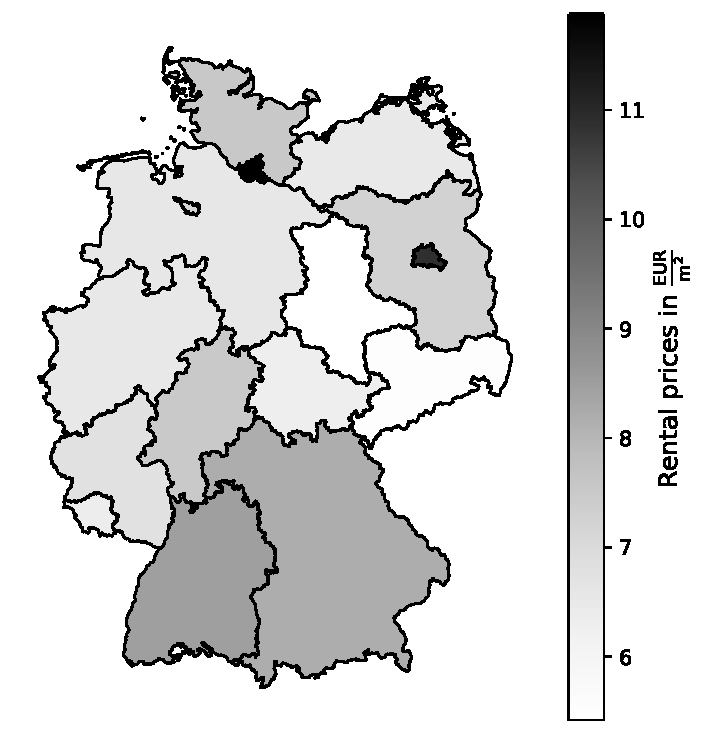
\includegraphics[width=0.5\linewidth]{../fig/figures/geodata_2017.pdf}
	\caption{Geopandas map depicting german states with their corresponding average rental prices. The visualisation shows again, that eastern states tend to have a lower average rental price in comparison to the west. Outstanding are the citystates Hamburg and Berlin, that show an extraordinary rental price. Geodata gained from \cite{geo_data}.}
	\label{geodata_2017}
	\end{figure}
	\newpage
	
	
	
	
	\section{Discussion and Limitations}
	\label{limitations}
	Of course a serious limitation that becomes significant to the results given in \cref{results} is the lack of input data. In general, the amount of data lacks especially in the years ranging from 2002 to 2010. But also when analyzing data from 2010 and further it is striking that the standard deviation is very high on a relative scale.\\\\
	Taking the values for 2017, for instance, the standard deviation is approx. 25 \% on the raw dataset (cities), see \cref{Table_raw}. This can have multiple reasons. Of course germany has regions of high income, as well as regions of rather low income. Hence, as a natural consequence, the standard deviation, taking the spread of high priced areas and low ones into account, displays that differences. Furthermore, it is not clear how the data itself got generated, so it is possible that errors occur on a regular basis, which is not possible to find out in the analysis. Also it is important to say, that the values for Hamburg and Berlin, being citystates are not directly comparable to the rest of the data, because there has been only one data point reported, respectively.\\\\
	In addition to that, it is important to take into account, that although data from 2011 has been used to compare the current rental prices from 2017, there is a difference of about 100 data points between these two datasets. Hence, a portion of the "mass-shift" described in \cref{histogram_rental_prices} can be explained with that fact, although the remaining shift is still significant enough to draw the conclusions described in \cref{results}. \\\\
	In general a conclusion that high priced rental cities are located in Bavaria in comparison to other german states is problematic, because it is possible that the dataset contains more data from bavarian cities than from cities located in other states. In fact this is the case, which can be seen in \cref{Table_bavarian_cities}. Still, the conclusion is still correct, concerning other sources, that Munich is the highest priced city (neglecting islands) and therefore city parts of Munich are also the most expensive regions.\cite{munich_prices}\\\\
	However, the analysis takes Baden-Württemberg and Bayern in "advantage", because more data points got aquired in the process for those two states. The same argument is true for a comparison between eastern and western states. Far more data has been collected for western cities than it has been for eastern ones. This conclusion can be drawn from \cref{Table_bavarian_cities}, where approx. 2 000 data points have been collected for western countries, whereas only approx. 300 have been counted for the eastern states.
	\newpage
		\renewcommand{\arraystretch}{1.3}
		\begin{table}[h!]
			\caption{Number of collected data points for the years of interest 2010 and 2017. It is significant that especially Baden-Württemberg and Bayern are providing most data, therefore it becomes obvious that these two appear more often in the analysis than the other states.}
			\label{Table_bavarian_cities}
			\centering
			\begin{tabular}{lrr}
\toprule
{} &  data points 2017 &  data points 2010 \\
state                  &                   &                   \\
\midrule
Baden-Wuerttemberg     &               373 &               352 \\
Bayern                 &               623 &               587 \\
Berlin                 &                 1 &                 1 \\
Brandenburg            &                41 &                30 \\
Bremen                 &                 2 &                 2 \\
Hamburg                &                 1 &                 1 \\
Hessen                 &               215 &               212 \\
Mecklenburg-Vorpommern &                40 &                24 \\
Niedersachsen          &               225 &               197 \\
Nordrhein-Westfalen    &               303 &               301 \\
Rheinland-Pfalz        &               131 &               119 \\
Saarland               &                29 &                29 \\
Sachsen                &               113 &                99 \\
Sachsen-Anhalt         &                47 &                45 \\
Schleswig-Holstein     &               127 &               102 \\
Thueringen             &                47 &                23 \\
\bottomrule
\end{tabular}

		\end{table}
	\label{outlook}
\bibliography{ref.bib}

\end{document}
